%============================================================================
% Example for EVGA 2021 proceedings
%
% OBS: Do not change anything in this upper part of the file
%
%============================================================================
\documentclass[natbib,twocolumn,twoside]{svmultiag}
\usepackage{graphicx}
%- - - - - - - - - - - - - - - - - - - - - - - - - - - - - - - - - - -
% OBS: if you have special packages that you need, then add them below
%
% special LaTeX packages needed are:
%- - - - - - - - - - - - - - - - - -
% \usepackage{...}
\usepackage{pdfpages}
\usepackage[english]{babel}
\usepackage[latin1]{inputenc}
\usepackage{caption}
\usepackage[normalem]{ulem}
\usepackage{multicol}
\usepackage{vwcol}
\usepackage{multirow}
\usepackage{tabularx}
\usepackage{subfig}
\usepackage{makecell}
\usepackage{url}
\newcolumntype{C}{>{\centering\arraybackslash}X}
\newcolumntype{Y}{<{\centering\arraybackslash}Y}
%============================================================================
%------------------------------------------------------------------------------
%
% HERE COME TITLE AND AUTHORS
%
%------------------------------------------------------------------------------
\title*{First results from the new station NYALE13S}
\titlerunning{NYALE13S - First results}

\author{A-S.~Kirkvik, M.,~D\"ahnn, I.~Fausk}
\authorrunning{Kirkvik et al.}

\institute{Ann-Silje Kirkvik \and Michael D\"ahnn \and Ingrid Fausk
\at Kartverket,
Postboks 600 Sentrum,
3507 H\o nefoss,
Norway
}
%============================================================================
%
% HERE BEGINS THE MAIN TEXT
%
\begin{document}
\maketitle
\thispagestyle{empty}
\pagestyle{empty}
%----------------------------------------------------------------------------
\abstract{
In February 2020 the new VLBI station NYALE13S had its first successful 24 hour session with a tri-band receiver.
The goal is to have at least one and a half year of parallel observations with NYALE13S and NYALES20.
The purpose of the legacy observations is to be able to transfer the long time series from 
NYALES20 to the new station NYALE13S and compare the results with the local tie measurements.
The length of the NYALES20-NYALE13S baseline is approximately 1.5 kilometers. There are at the moment
17 sessions available with observations from both NYALE13S and NYALES20. These and future parallel
observations will be very useful for connecting future VGOS observations with the legacy
network. The baseline length estimated from VLBI observations agree well with the local tie measurements,
but the uncertainty is high. The number of available observations is significantly less than scheduled due to problems with
the equipment both at the new and old station. The results are therefore very preliminary and
hopefully more sessions will be observed in the near future. 
}

\keywords{VLBI, Baseline length, Ny-\AA lesund}

%----------------------------------------------------------------------------
\section{Introduction}                                
\label{sec:introduction}
%----------------------------------------------------------------------------
The road from the inauguration of the new geodetic observatory in Ny-\AA lesund in June 2018 to making the first successful
analysis of recorded data has been long and filled with problems. But the station NYALE13S is finally recording usable 
data. The station is equipped with a tri-band receiver and will participate in R1 and R4 sessions 
together with NYALES20 before NYALES20 is dismantled and NYALE13S is equipped with a 
broadband receiver. 

NYALE13S joined as tag-along for R1 sessions in July 2019 but the first fringe was not found until December 2019. 
And it was not until February 2020 multiple fringes were found and the data could be analysed. These first few sessions with
data from both the new station NYALE13S (Ns) and the old station NYALES20 (Ny) have been analyzed and results are compared to the 
preliminary results from the local tie measurements.

%............................................................................
% FIG:01 START
%............................................................................
%\begin{figure}[t!]
%\includegraphics[width=0.5\textwidth]{blabla.pdf}
%\caption{
%Blabla blublu bloblo
%blabla blublu bloblo
%blabla blublu bloblo
%blabla blublu bloblo
%blabla blublu bloblo.}
%\label{FIG:blabla blublu bloblo}
%\end{figure}
%............................................................................
% FIG:01 END
%............................................................................

%----------------------------------------------------------------------------
\section{Data}                                 
\label{sec:data}
%----------------------------------------------------------------------------

On the 17th of February 2020 the new station NYALE13S had its first
successful 24 hour session. The week before some data was successfully correlated,
but since it was only 88 observations spanning 3 hours the station was not included 
in the official database. There is still only a limited number of sessions available 
with observations from both NYALE13S and NYALES20. The few sessions that 
exist are used in this analysis and are listed in table \ref{tab:sessions}. The sessions with only one of the
stations observing have also been analyzed, but those sessions are naturally not used in the analysis of 
baseline length and baseline length repeatability.

Numerous problems and issues occurred at both stations, which has affected the overall data
quality and availablity. First of all, NYALE13S has been scheduled as a tag-along
station for all these sessions. The station also observed with a warm receiver until R1945.
However, the SEFD values used in 
the schedule were not updated to reflect the cold receiver until R1947. At the same time the receiver
at NYALES20 started to heat up and the station observed with a warm receiver for the
remaining sessions.  

NYALE13S originally used a DBBC3 and FlexBuff system to record data. After a while the DBBC3 malfunctioned and had 
to be sent for repairs. The DBBC3 was
later replaced with a new DBBC2, but by then the elevation encoder at NYALES20 had
malfunctioned and also had to be sent for repairs. The elevation encoder was eventually fixed and
NYALES20 started observing again for R1995 but as tag-along and with a warm receiver. 

Shortly afterwards,
the phase calibration unit at NYALE13S malfunctioned during the R1996 experiment. The phase calibration unit is now replaced
but no more sessions have been recorded and correlated at the time of writing.  From R1997 and onwards NYALES20
is no longer in tag-along and the receiver will be cooled shortly. In addition, some individual sessions failed to 
record any usable data for NYALE13S. These sessions are not included in table \ref{tab:sessions}.

\begin{table}
\captionsetup{labelfont={color=black}}
	\begin{tabularx}{\columnwidth}{X|X|X|X}
	Session & Date & Warm & Tag-along\\
	\hline
	R1934 & 2020 02 17 & Ns & Ns\\
	R1935 & 2020 02 24 & Ns & Ns\\
	R1936 & 2020 03 02 & Ns & Ns\\
	R1937 & 2020 03 09 & Ns & Ns\\
	%\sout{R1938} & \sout{2020 03 16} \\
	R1939 & 2020 03 23 & Ns & Ns\\
	R1940 & 2020 03 30 & Ns & Ns\\
	%\sout{R1941} & \sout{2020 04 06} \\
	%\sout{R1942} & \sout{2020 04 14} \\
	%\sout{R1943} & \sout{2020 04 20} \\
	R1944 & 2020 04 27 & Ns & Ns\\
	R1945 & 2020 05 04 & Ny & Ns\\
	R1946 & 2020 05 11 & Ny & Ns\\
	R1947 & 2020 05 18 & Ny & Ns\\
	R1948 & 2020 05 26 & Ny & Ns\\
	R1949 & 2020 06 02 & Ny & Ns\\
	%\sout{R1950} & \sout{2020 06 08} \\
	R1951 & 2020 06 15 & Ny & Ns\\
	R1952 & 2020 06 22 & Ny & Ns\\
	R1995 & 2021 04 19 & Ny & Ns, Ny\\
	R4995 & 2021 04 22 & Ny & Ns, Ny\\
	R1996 & 2021 04 26 & Ny & Ns, Ny\\
	\hline
	\end{tabularx}
\caption{{Sessions used in analysis of baseline length between NYALE13S and NYALES20. The last two columns summarize the 
receiver temperature and tag-along status for both stations.}}
\label{tab:sessions}
\end{table}


%............................................................................
% TAB:01 START
%............................................................................
%\begin{table}
%\centering
%\caption{blabla blublu bloblo}
%\begin{tabular}{lll}
%\hline
%blabla & blublu & bloblo \\
%\hline
%1 & 2 & 3 \\
%3 & 2 & 1 \\
%2 & 3 & 1 \\
%\hline
%\end{tabular}
%\label{TAB: blabla}
%\end{table}
%............................................................................
% TAB:01 END
%............................................................................

%---------------------------------------------------------------------------
\section{Analysis}                                         
\label{sec:analysis}
%---------------------------------------------------------------------------
Multiple solutions were tested to see how the parameterization might affect the final results. The number of observations
available from NYALE13S is very limited and the quality is for the most part poor due to the warm receiver and other
problems with the sessions. This lowers the degrees of freedom and increases the uncertainty in the estimates. Different
setups for troposphere parameterizations and fixing the celestial reference frame have been tested.

The analysis has been done using \textbf{Where} (see \cite{hjelle2018}). The default solution is the same that is used for 
regular R1 and R4 processing. This means all station and source coordinates, EOPs, clocks and troposphere are estimated. 
For more information see \cite{kirkvik2017b} and \cite{kirkvik2019}. A priori coordinates for NYALE13S used in the 
analysis are computed based on the local 
tie vector since the coordinates in the original database is off by almost a meter. The baseline length and repeatability 
is calculated according to \cite{hofmeister2016}.

For comparision the same analysis is done for the baseline between 
WETTZELL (Wz) and WETTZ13N (Wn) with sessions from 2015 and 2016 when the WETTZ13N station was new. The local tie vector 
between WETTZELL and WETTZ13N is taken from \cite{schuler2018}. This baseline is almost 10 times shorter than the 
NYALES20/NYALE13S baseline, but both baselines are considered short in geodetic VLBI. This is a useful comparison since
both locations routinely participate in the R1 and R4 sessions and should be affected by the same network effects.


Figure \ref{fig:num_obs} shows the number of observations
used in each session for the NYALES20/NYALE13S baseline. The baseline length results are summarized in table 
\ref{tab:solutions} and selected plots are shown in figure \ref{fig:bl}, \ref{fig:sta} and \ref{fig:zwd}.  


\begin{figure}
	\subfloat[\textcolor{black}{Number of observations - NYALE13S}.\label{fig:num-Ns-0}]
      {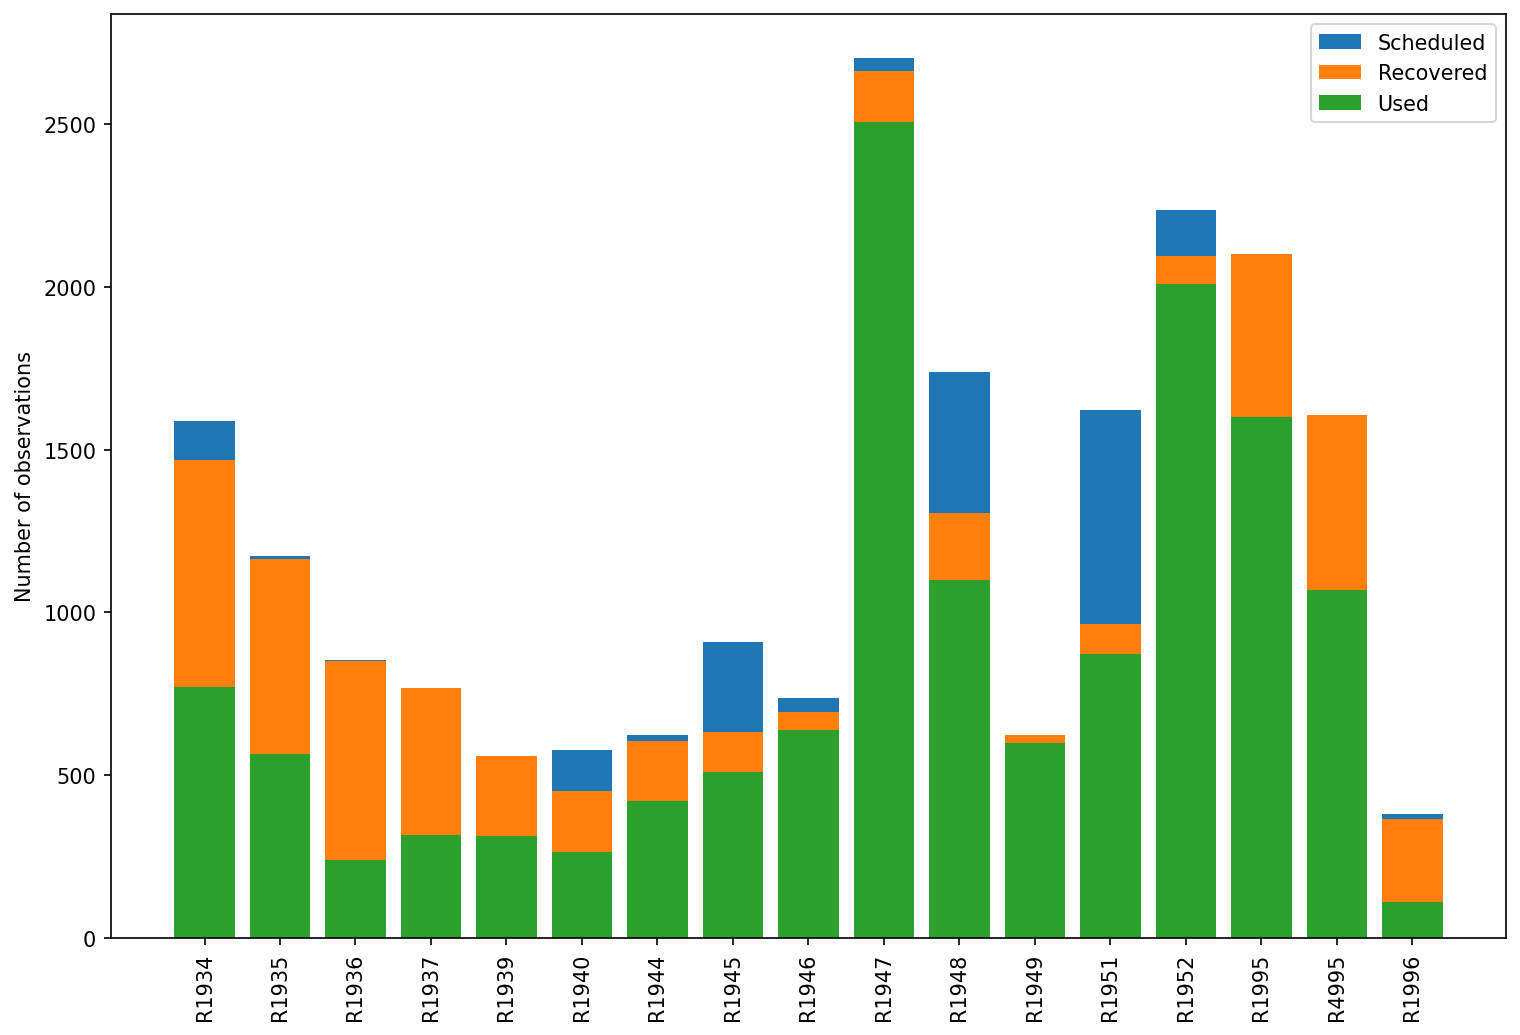
\includegraphics[width=\linewidth]{figure/Num_obs_NYALE13S_nyale13s0}} \\
    % Number of observations NYALES20
	\subfloat[\textcolor{black}{Number of observations - NYALES20}.\label{fig:num-Ny-0}]
      {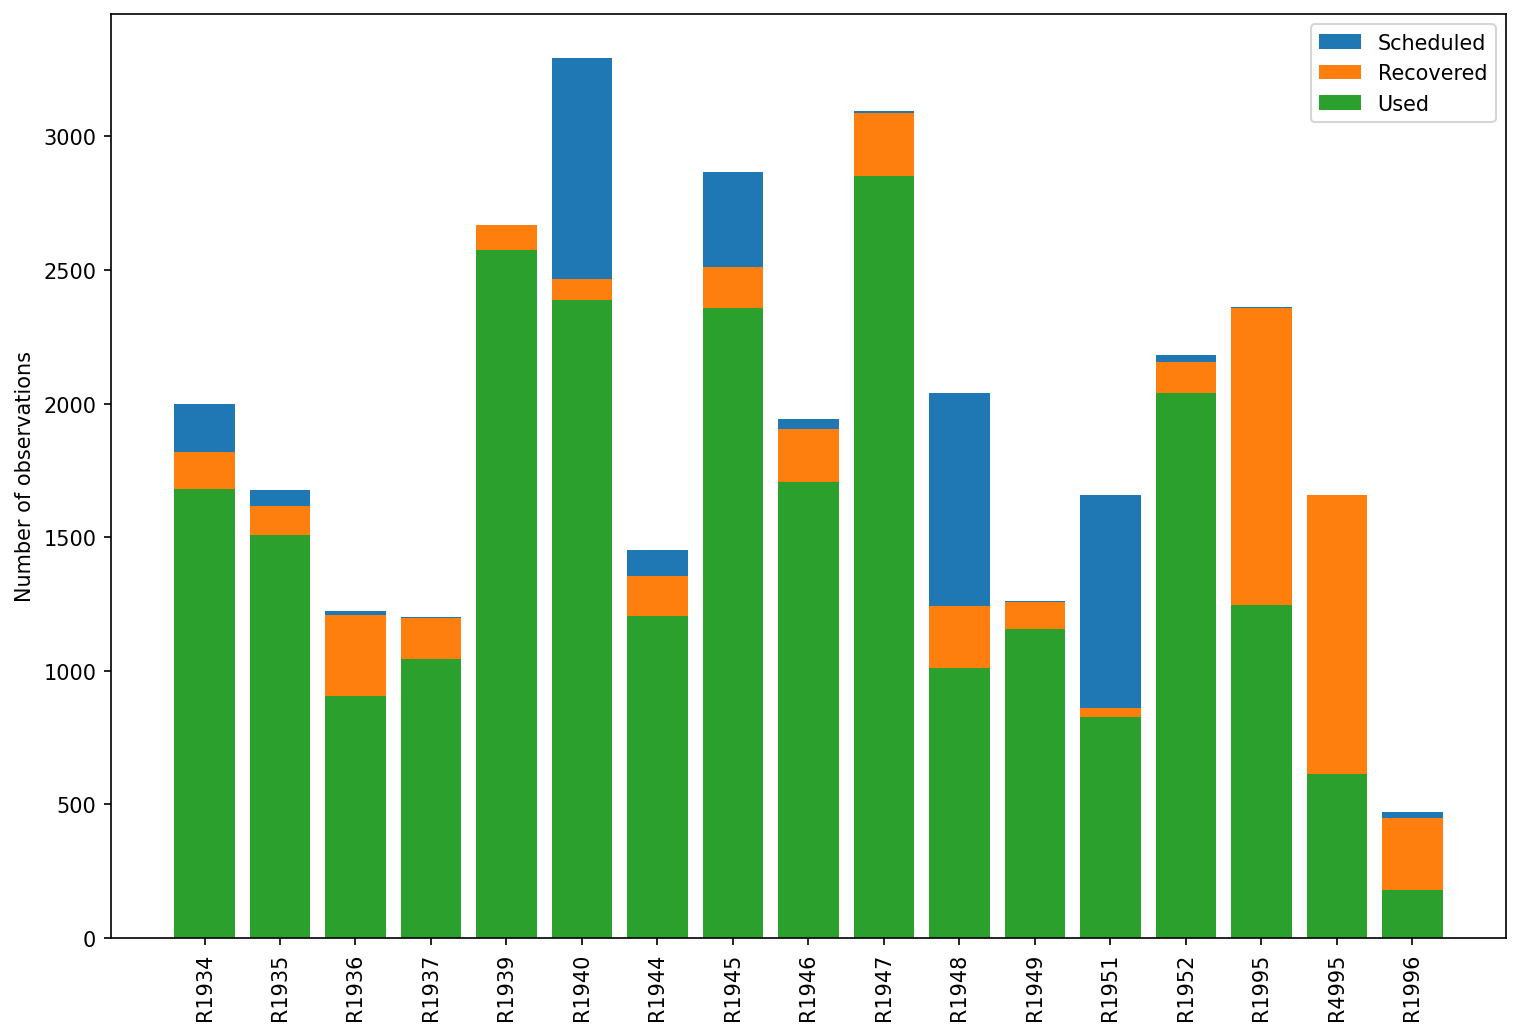
\includegraphics[width=\linewidth]{figure/Num_obs_NYALES20_nyale13s0}} \\
    %
    \caption{Number of observations available from NYALES20 (\ref{fig:num-Ns-0}) and NYALE13S (\ref{fig:num-Ny-0}) 
    for the sessions with both stations participating.
    The blue bar is the number of scheduled observations. The orange bar is the number of observations successfully 
    recovered at the correlator and the green bar is the number of observations used in the analysis. The plots are from 
    solution 0.}
	\label{fig:num_obs}
\end{figure}

%% nyale13s0: Weighted mean:  1539.1931 [m], Local tie offset:  0.0000 [m]
%% nyale13s0: Weighted blr (using weighted mean):  0.0033 [m]
%% nyale13s1: Weighted mean:  1539.1944 [m], Local tie offset:  0.0013 [m]
%% nyale13s1: Weighted blr (using weighted mean):  0.0025 [m]
%% nyale13s2: Weighted mean:  1539.1927 [m], Local tie offset: -0.0004 [m]
%% nyale13s2: Weighted blr (using weighted mean):  0.0032 [m]
%% nyale13s3: Weighted mean:  1539.1943 [m], Local tie offset:  0.0012 [m]
%% nyale13s3: Weighted blr (using weighted mean):  0.0023 [m]
%% nyale13s4: Weighted mean:  1539.1924 [m], Local tie offset: -0.0007 [m]
%% nyale13s4: Weighted blr (using weighted mean):  0.0029 [m]
%% nyale13s5: Weighted mean:  1539.1938 [m], Local tie offset:  0.0007 [m]
%% nyale13s5: Weighted blr (using weighted mean):  0.0023 [m]
%% nyale13s6: Weighted mean:  1539.1946 [m], Local tie offset:  0.0015 [m]
%% nyale13s6: Weighted blr (using weighted mean):  0.0025 [m]
%% nyale13s7: Weighted mean:  1539.1927 [m], Local tie offset: -0.0004 [m]
%% nyale13s7: Weighted blr (using weighted mean):  0.0034 [m]
%% nyale13s8: Weighted mean:  1539.1945 [m], Local tie offset:  0.0014 [m]
%% nyale13s8: Weighted blr (using weighted mean):  0.0023 [m]
%% nyale13s9: Weighted mean:  1539.1925 [m], Local tie offset: -0.0006 [m]
%% nyale13s9: Weighted blr (using weighted mean):  0.0028 [m]
%%wettzell0: Weighted mean:  123.3064 [m], Local tie offset: -0.0006 [m]
%%wettzell0: Weighted blr (using weighted mean):  0.0017 [m]

 

\begin{table*}[t]
\captionsetup{labelfont={color=black}}
	\begin{tabularx}{\textwidth}{l|l|X|c|c|c}
	~\#~ & ~Baseline~ & ~Setup~ & WBL & WBLR & dL \\
	\hline
	~0~ & ~Ns-Ny~ & ~\makecell[tl]{Default}~ & ~1539.1931 [m]~ & ~0.0033 [m]~ & ~~0.0000 [m]~ \\
	~1~ & ~Ns-Ny~ & ~\makecell[tl]{Troposphere gradients fixed (Ns)}~ & ~1539.1944 [m]~ & ~0.0025 [m]~ & ~~0.0013 [m]~ \\ 
	~2~ & ~Ns-Ny~ & ~\makecell[tl]{Troposphere gradients fixed (Ns and Ny) \\ 
	Zenith wet delay fixed (Ns and Ny)}~ & ~1539.1927 [m]~ & ~0.0032 [m]~ & ~-0.0004 [m]~ \\ 
	~3~ & ~Ns-Ny~ & ~\makecell[tl]{Troposphere gradients fixed (Ns) \\ 
	Two hour zenith wet delay (Ns)}~ & ~1539.1943 [m]~ & ~0.0023 [m]~  & ~~0.0012 [m]~ \\
	~4~ & ~Ns-Ny~ & ~\makecell[tl]{Troposphere gradients fixed (Ns and Ny) \\ 
	Two hour zenith wet delay (Ns and Ny)}~ & ~1539.1924 [m]~ & ~0.0029 [m]~ & ~-0.0007 [m]~ \\
	~5~ & ~Ns-Ny~ & ~\makecell[tl]{Radio sources fixed}~ & ~1539.1938 [m]~ & ~0.0023 [m]~ & ~~0.0007 [m]~ \\
	~6~ & ~Ns-Ny~ & ~\makecell[tl]{Radio sources fixed \\ 
	Troposphere gradients fixed (Ns)}~ & ~1539.1946 [m]~ & ~0.0025 [m]~ & ~~0.0015 [m]~ \\
	~7~ & ~Ns-Ny~ & ~\makecell[tl]{Radio sources fixed \\ 
	Troposphere gradients fixed (Ns and Ny) \\ 
	Zenith wet delay fixed (Ns and Ny)}~  & ~1539.1927 [m]~ & ~0.0034 [m]~ & ~-0.0004 [m]~ \\
	~8~ & ~Ns-Ny~ & ~\makecell[tl]{Radio sources fixed \\ 
	Troposphere gradients fixed (Ns) \\ 
	Two hour zenith wet delay (Ns)}~ & ~1539.1945 [m]~ & ~0.0023 [m]~ & ~~0.0014 [m]~ \\
	~9~ & ~Ns-Ny~ & ~\makecell[tl]{Radio sources fixed \\ 
	Troposphere gradients fixed (Ns and Ny) \\ 
	Two hour zenith wet delay (Ns and Ny)}~ & ~1539.1925 [m]~ & ~0.0028 [m]~ & ~-0.0006 [m]~ \\
	~10~ & ~Wn-Wz~ & ~\makecell[tl]{Default}~ & ~~123.3064 [m]~ & ~0.0017 [m]~ & ~-0.0006 [m]~ \\
	\hline
	\end{tabularx}
\caption{{Weighted baseline length (WBL), weighted baseline length repeatability (WBLR) and difference 
between weighted baseline length and local tie vector (dL) for the different solutions. The third column described how 
a solution differs from the default solution.
}}
\label{tab:solutions}
\end{table*}

\begin{figure}
    % Baseline lengths NYALE13S/NYALES20
	\subfloat[\textcolor{black}{Baseline length - NYALE13S/NYALES20}.\label{fig:bl-0}]
      {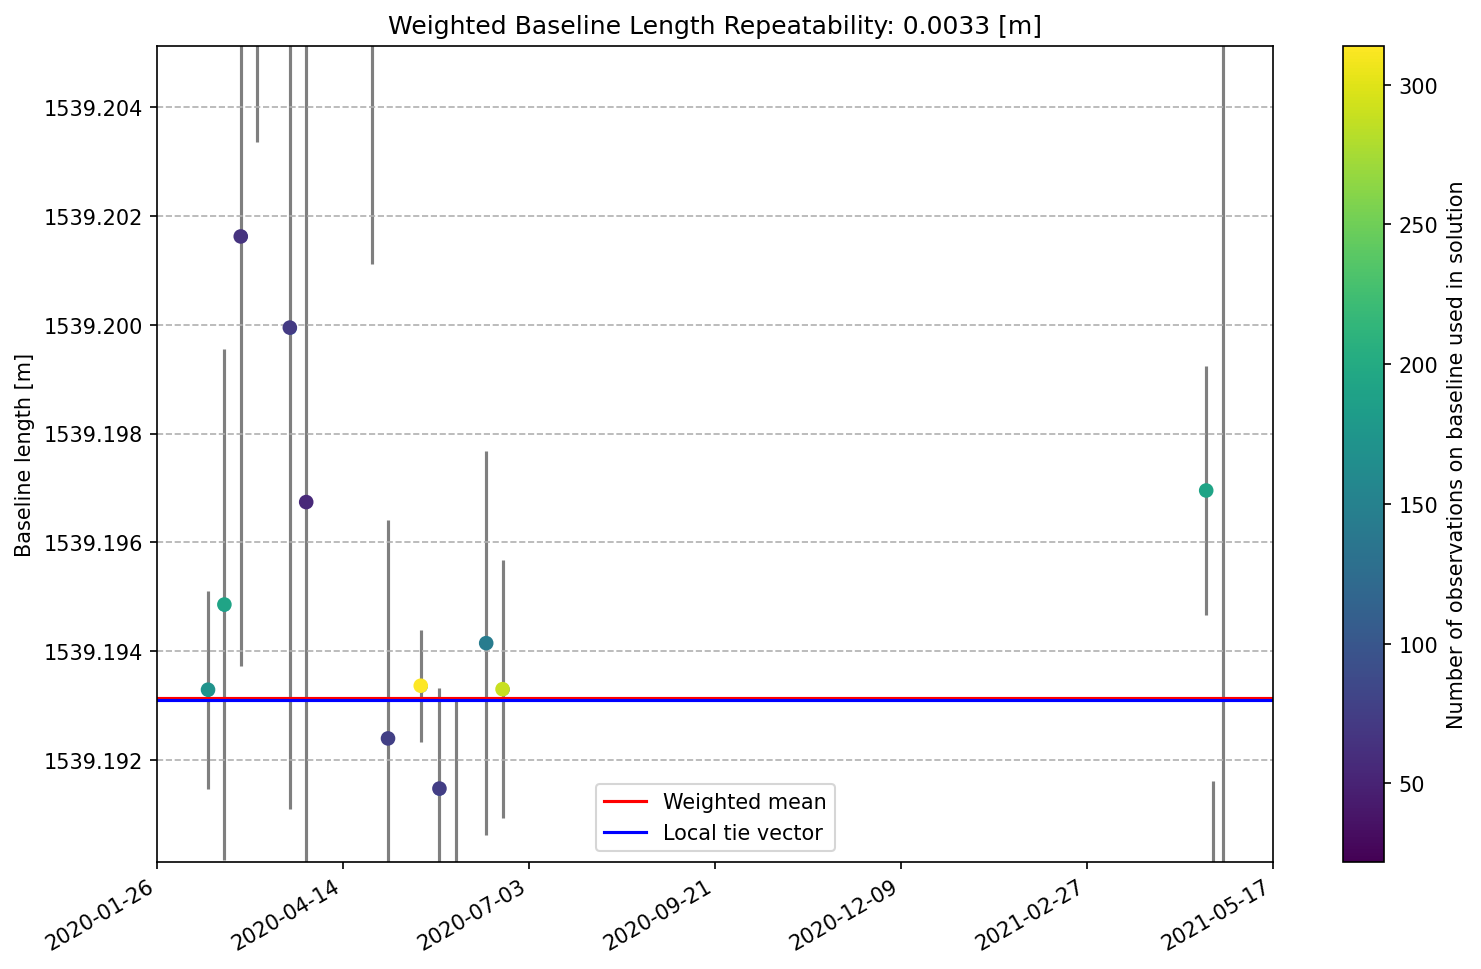
\includegraphics[width=\linewidth]{figure/Baseline_NYALES20_NYALE13S_nyale13s0}} \\
    % Baseline lengths WETTZELL/WETTZ13N
	\subfloat[\textcolor{black}{Baseline length - WETTZELL/WETTZ13N}.\label{fig:bl-10}]
      {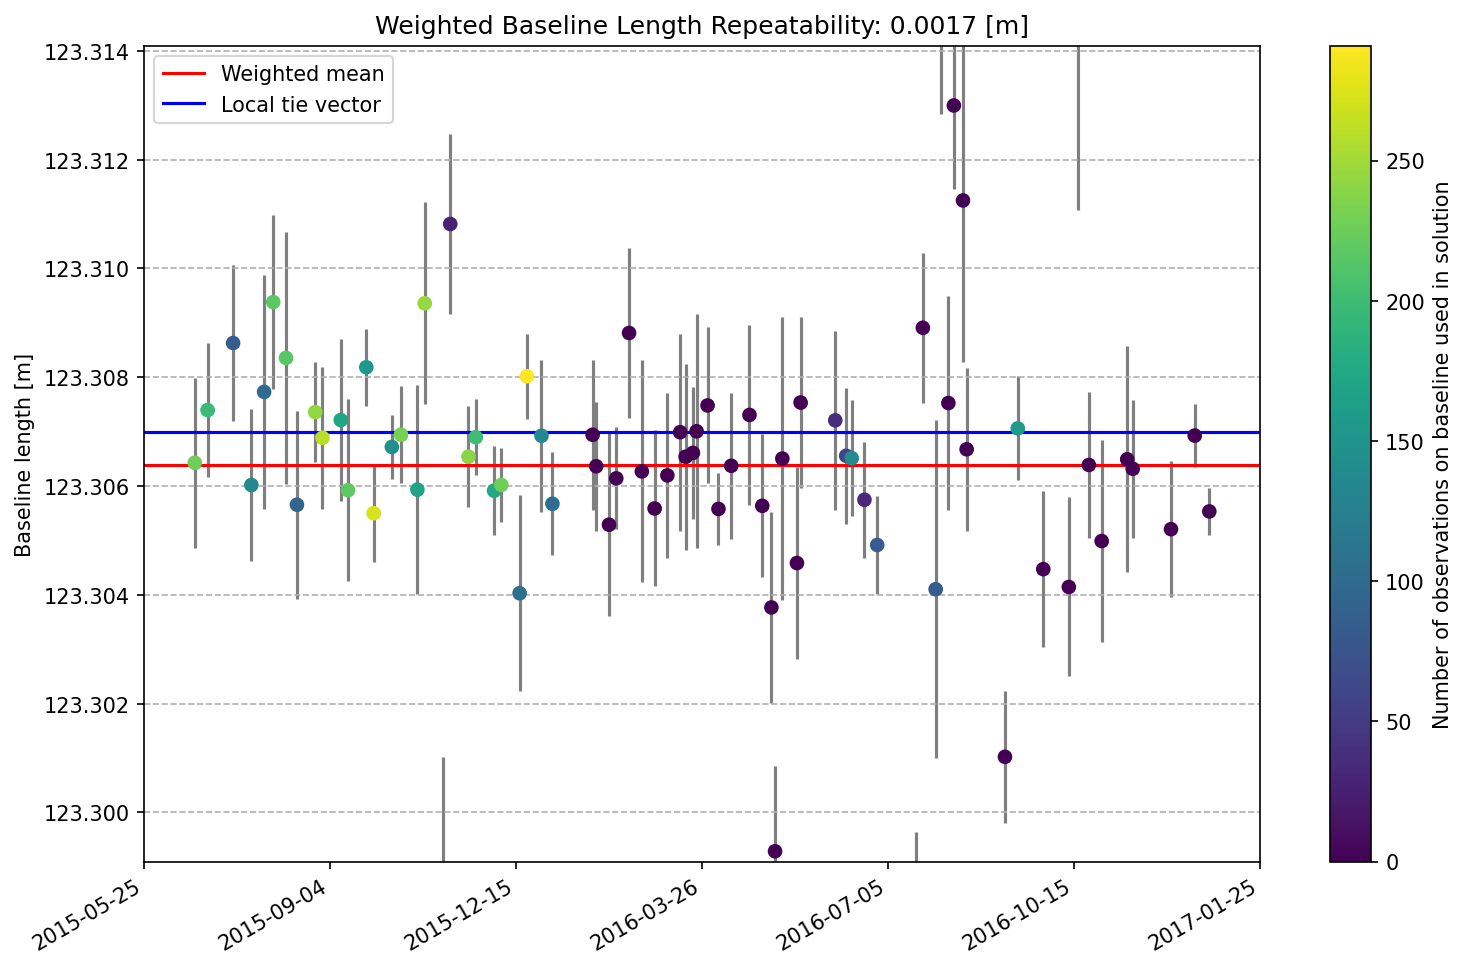
\includegraphics[width=\linewidth]{figure/Baseline_WETTZ13N_WETTZELL_wettzell0}} \\
    % Number of observations NYALE13S
    \caption{Estimated baseline lengths. The plot for the NYALES20/NYALE13S baseline (\ref{fig:bl-0}) is from 
    solution 0 and the plot for
    the WETTZELL/WETTZ13N baseline (\ref{fig:bl-10}) is from solution 10. Although the baseline length for the station pairs are different, the size of the vertical axis is the same for the two plots.}
	\label{fig:bl}
\end{figure}


\begin{figure}
    % Position NYALE13S
	\subfloat[\textcolor{black}{Estimated position - NYALE13S}.\label{fig:pos-Ns-0}]
      {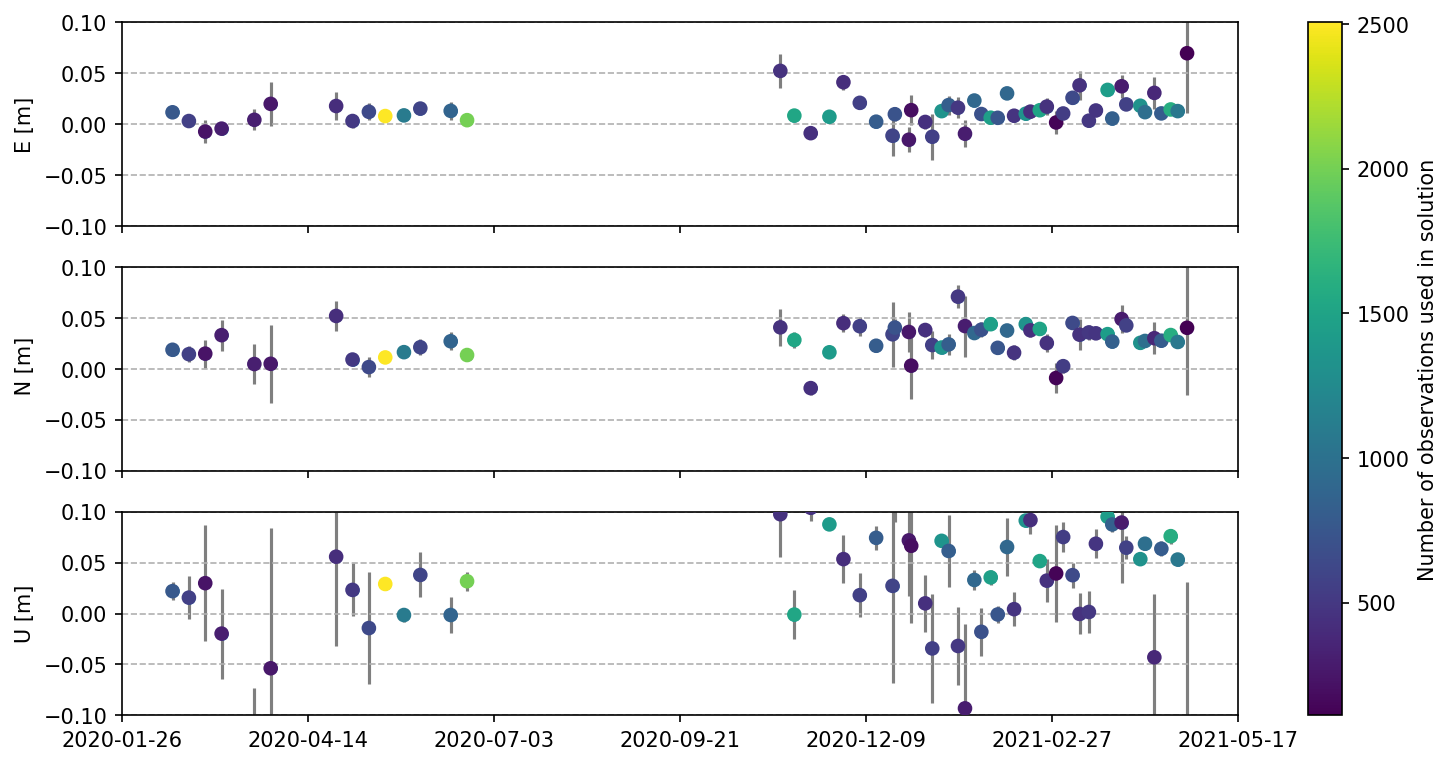
\includegraphics[width=\linewidth]{figure/Position_NYALE13S_enu_nyale13s0}} \\
    % Position NYALES20
	\subfloat[\textcolor{black}{Estimated position - NYALES20}.\label{fig:pos-Ny-0}]
      {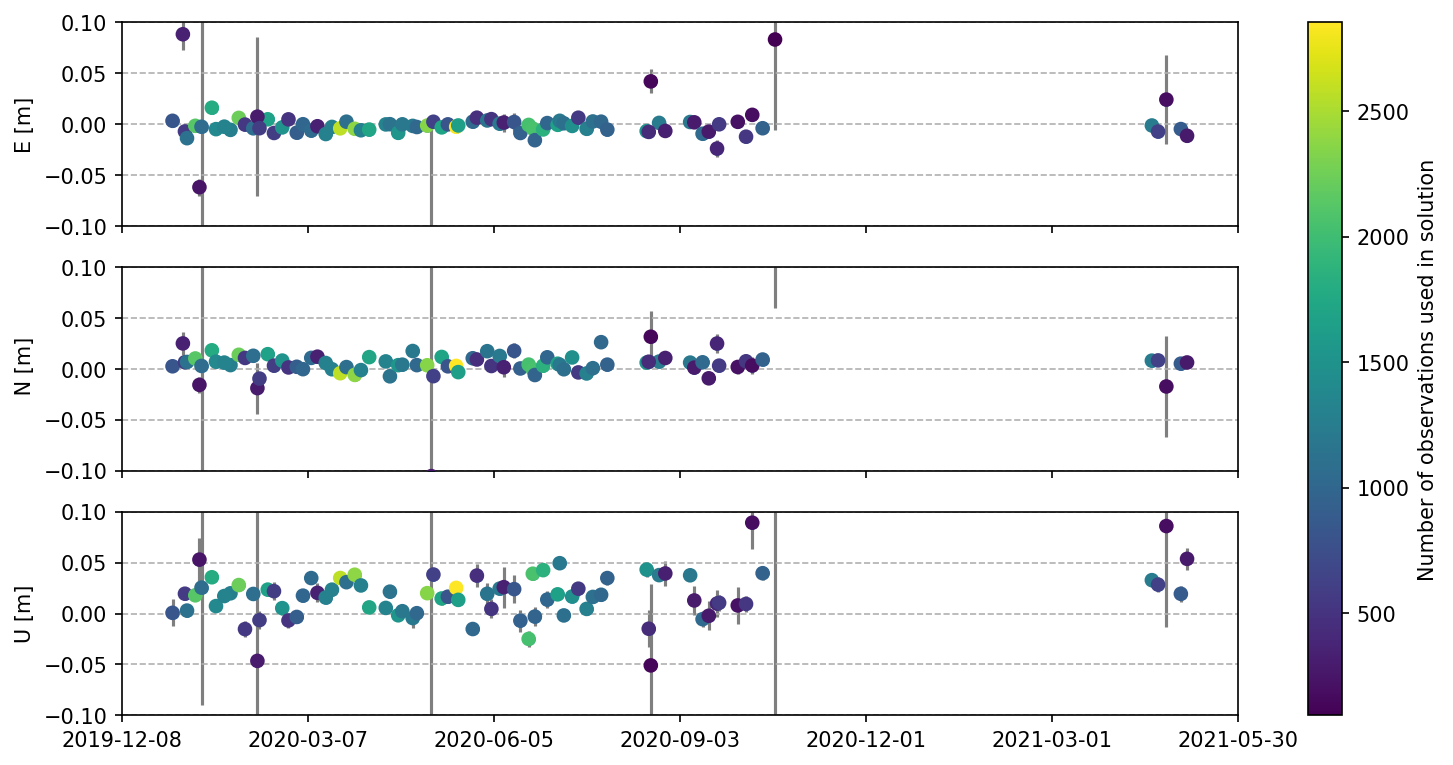
\includegraphics[width=\linewidth]{figure/Position_NYALES20_enu_nyale13s0}} \\ 
    % RMS
	\subfloat[\textcolor{black}{Root mean square of postfit residuals [m]}.\label{fig:rms-0}]
      {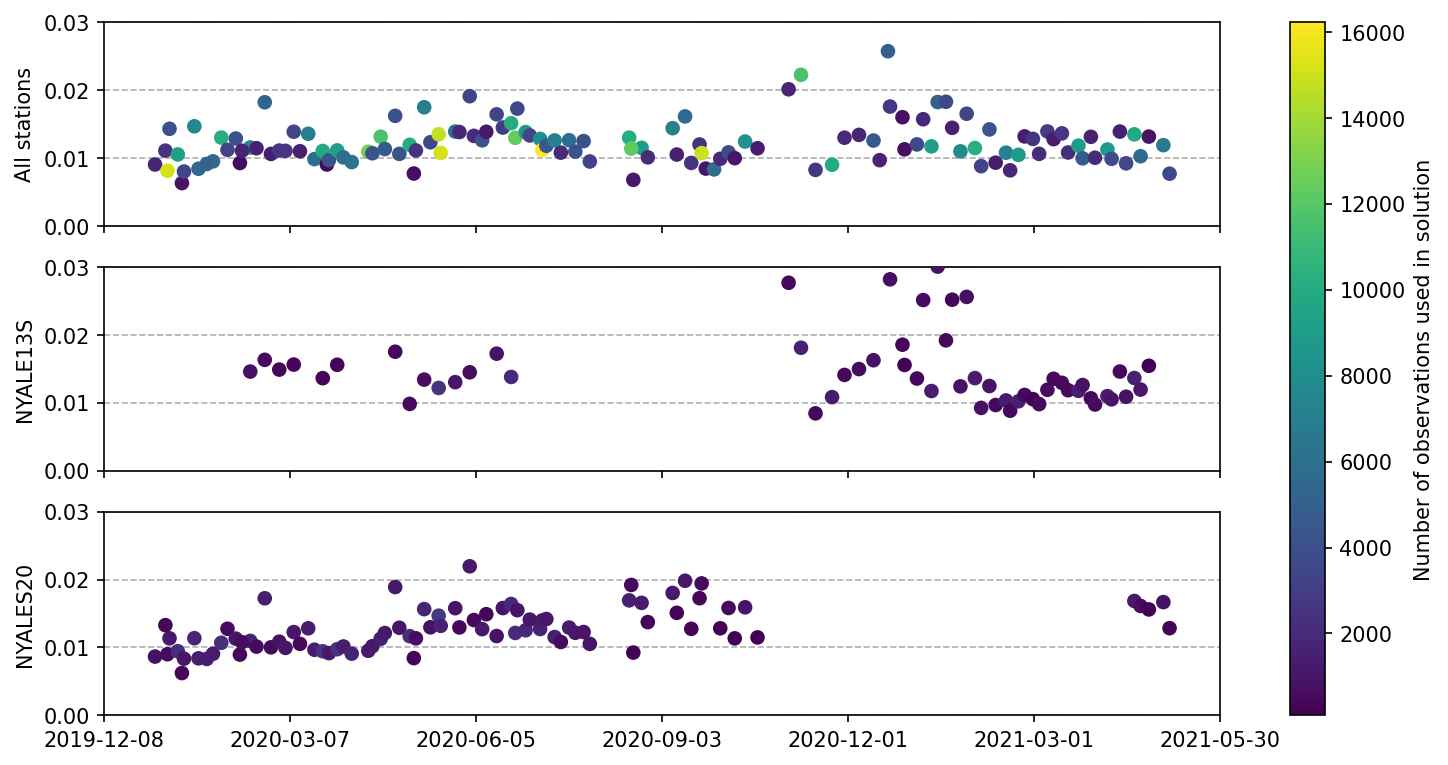
\includegraphics[width=\linewidth]{figure/RMS_Postfit_Residuals_nyale13s0}} \\
    % Statistics
%	\subfloat[\textcolor{black}{Statistics}.\label{fig:stat-0}]
%      {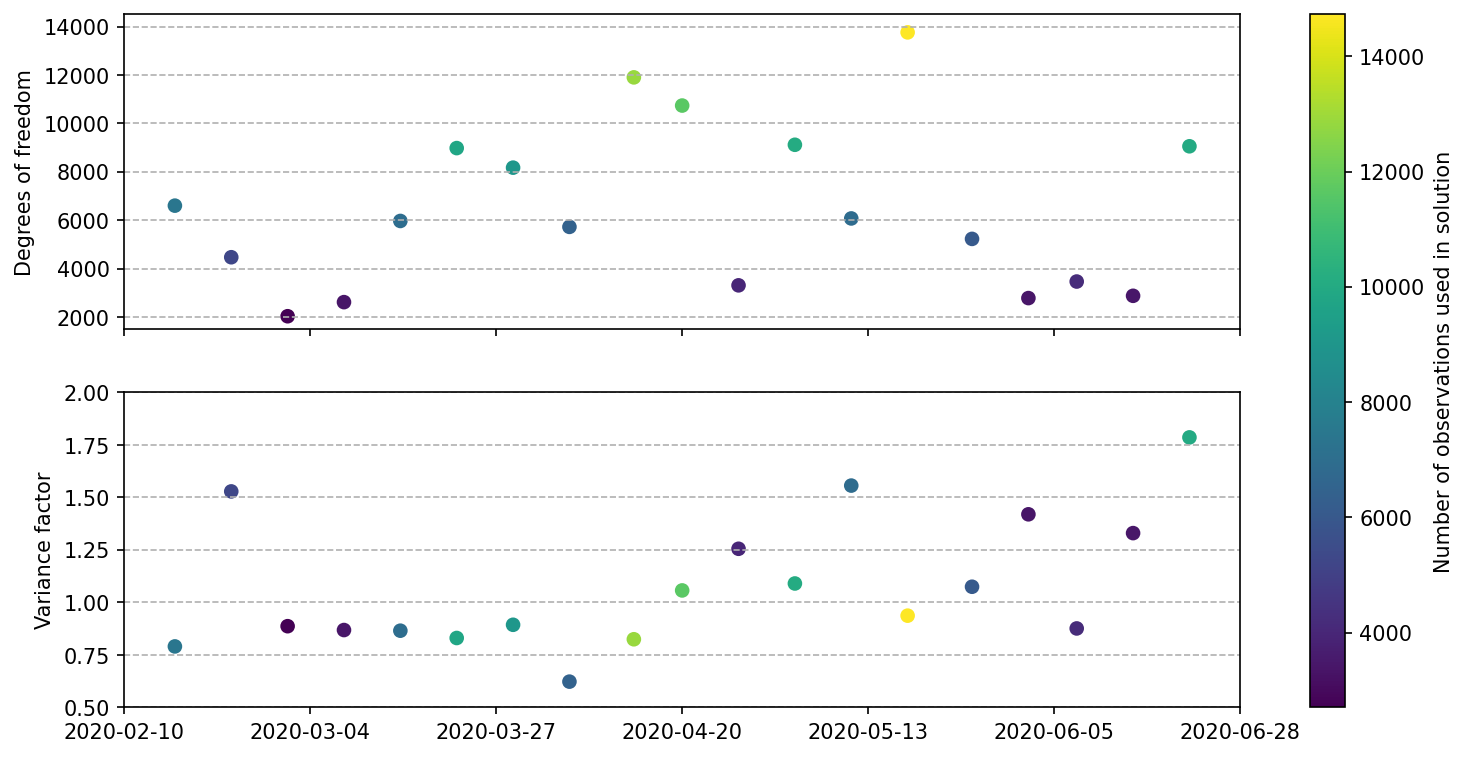
\includegraphics[width=\linewidth]{figure/Statistics_nyale13s0}} \\
    %  
	\caption{Estimated positions for NYALE13S (\ref{fig:pos-Ns-0}), NYALES20 (\ref{fig:pos-Ny-0}) and postfit residuals 
	(\ref{fig:rms-0}) for all sessions including either 
	NYALES20 or NYALE13S from 2020 until May 2021. The plots are from solution 0.}
	\label{fig:sta}
\end{figure}

\begin{figure}
	\subfloat[\textcolor{black}{Solution 0}.\label{fig:zwd0}]
	{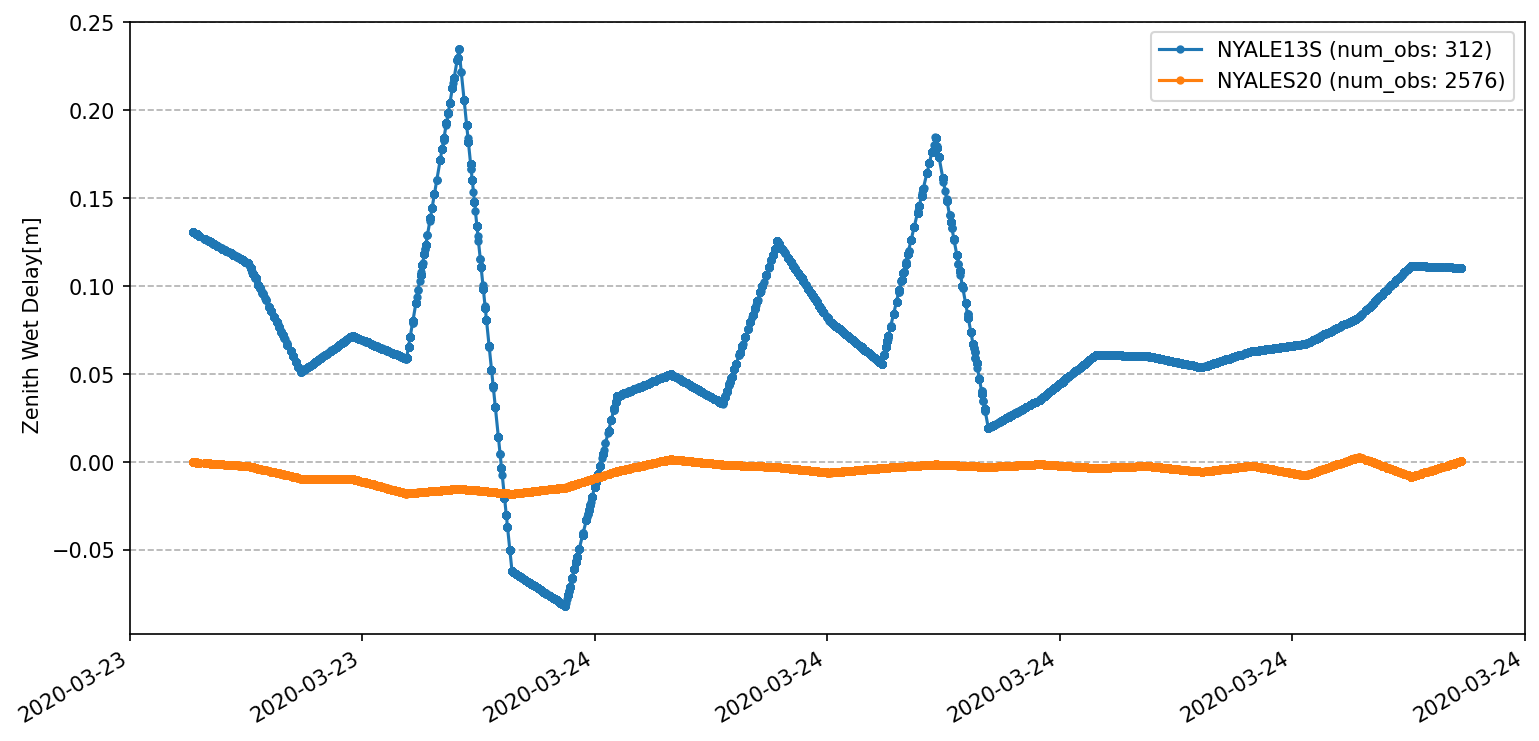
\includegraphics[width=\linewidth]{figure/Zenith_wet_delay_2020-03-23_XA_nyale13s0}} \\
	\subfloat[\textcolor{black}{Solution 9}.\label{fig:zwd9}]
	{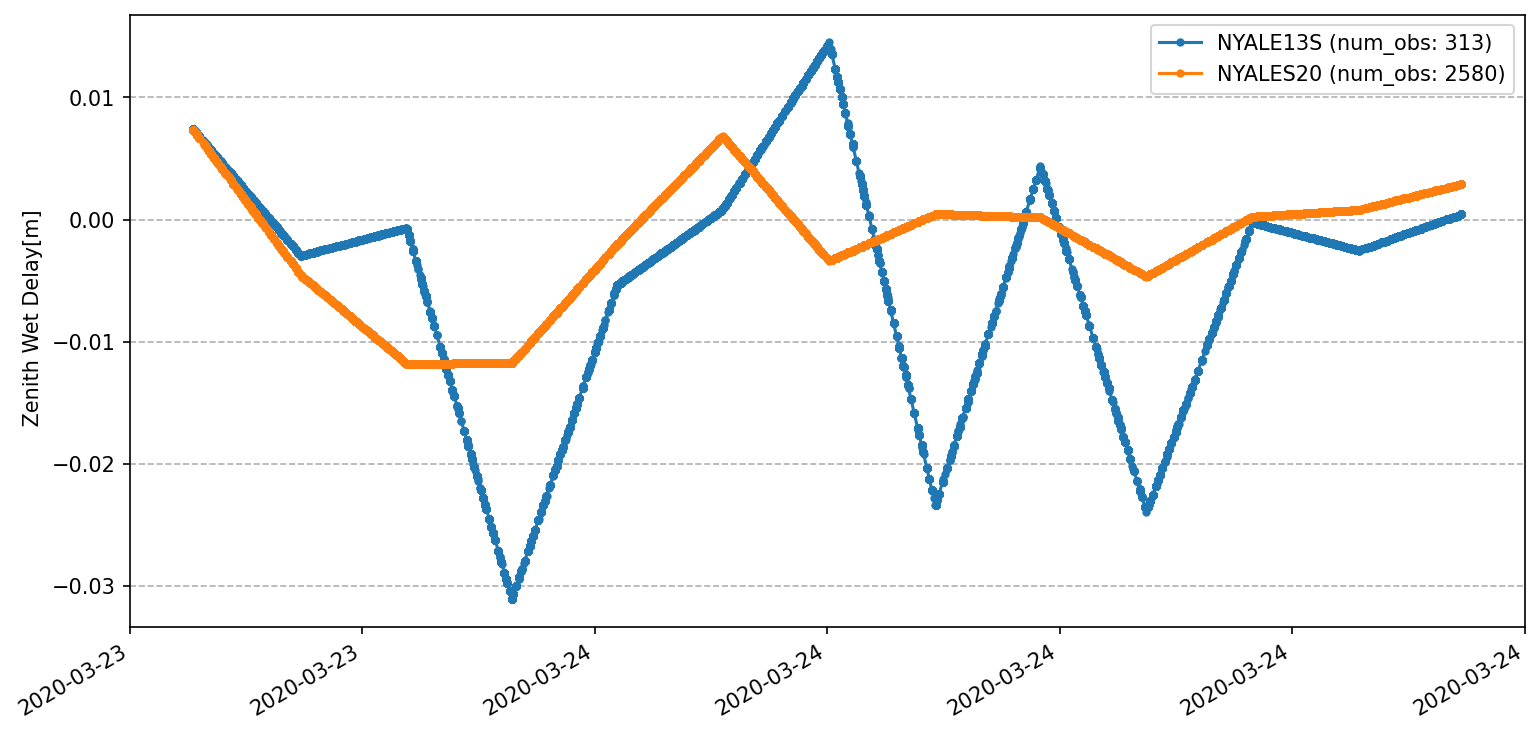
\includegraphics[width=\linewidth]{figure/Zenith_wet_delay_2020-03-23_XA_nyale13s9}} \\
	%
	\caption{Estimated correction to a priori zenith wet delay for R1939 for solution 0 (\ref{fig:zwd0}) and solution
	9 (\ref{fig:zwd9}). Notice the change in scale between solutions.}
	\label{fig:zwd}
\end{figure}


\section{Discussion} 
The length of the NYALES20/NYALE13S baseline 
vector is approximately 1.5km and there is a height difference between the stations of approximately
33 meters. In addition, the NYALE13S is very close to the coast. Are these stations close
enough to experience the same troposphere? The baseline length seem to agree better with the local tie
vector if the troposphere is treated the same at both stations. But the repeatability is poor and
the number of sessions available are low. As can been seen in \ref{fig:sta}, the uncertainty is mostly due to the perfomance of 
NYALE13S. 

The worst solutions in terms of baseline length repeatabilities are the solutions where the troposphere (both
gradients and zenith wet delay) are fixed to the a priori model. This seems to confirm the need to estimate
the troposphere parameters. 

The default solution is also one of the worst solutions. As can be seen in figure \ref{fig:zwd}, the low number of 
available
observations can cause the troposphere estimates to become unrealistic. This can be fixed by adding more constraints
to the solution or changing the parameterization, as is done in solution 9. Comparing troposphere estimates from the two
sites with estimates from GNSS receivers (figure \ref{fig:gnss}) confirms that the differences between the sites are lower than the 
differences in zenith wet delay from solution 0 for some sessions. The GNSS results are total tropospheric delay estimated 
every 2 hours and are not directly comparable to the zenith wet delay corrections from VLBI.    
 
It should be noted that the local tie vector is also just a preliminary result without known uncertainties at the moment. 


\section{Conclusions} 

The baseline length estimated from VLBI observations agree well with the local tie measurements, but the uncertainties are
high. \cite{nilsson2015} saw improvement in baseline length repeatabilites
for baselines shorter than 1km when assuming the troposphere at both stations were the same. The limited number of
observations available at NYALE13S causes high uncertainties in the position estimates and baseline lengths 
and the results might be improved by utilizing the troposphere information at NYALES20. Since the NYALES20/NYALE13S baseline
is longer than 1km, more work is needed to investigate this possibility.

The local tie computations need to be finalized and ultimately, more and better observations are needed
from the VLBI antennas. Only a few sessions have good quality and the weighted baseline
length repeatability would be significantly better if more sessions were of this quality. 

\begin{figure}
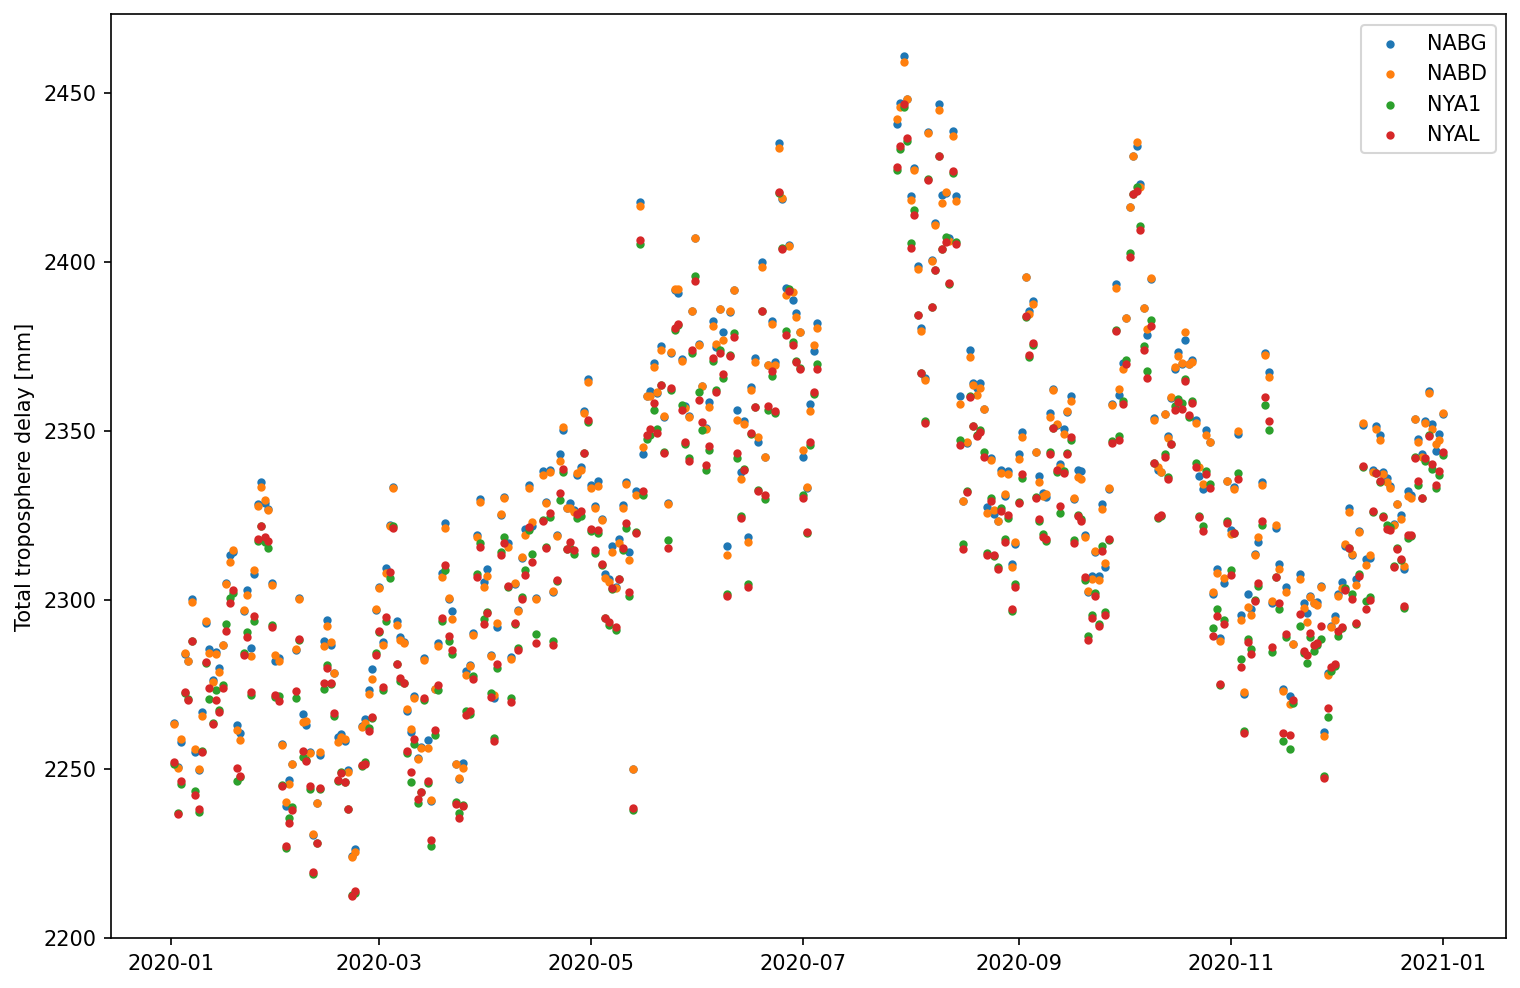
\includegraphics[width=\linewidth]{figure/GNSS_trop_tot}
\caption{Estimated total troposphere delay from four GNSS sites in Ny-\AA lesund in 2020. The results are produced with the GNSS
Bernese Software Version 5.2. NABG and NABD is located close to NYALE13S and NYAL and NYA1 is located close to NYALES20.}
\label{fig:gnss}
\end{figure}
%---------------------------------------------------------------------------
\begin{thebibliography}{99}
%--------------------------
\providecommand{\natexlab}[1]{#1}
\providecommand{\url}[1]{\texttt{#1}}
\expandafter\ifx\csname urlstyle\endcsname\relax
  \providecommand{\doi}[1]{doi: #1}\else
  \providecommand{\doi}{doi: \begingroup \urlstyle{rm}\Url}\fi

\bibitem[Hjelle et al. (2018)]{hjelle2018}
Hjelle, G.~A., Kirkvik, A.-S., D\"ahnn, M., Fausk, I. (2018)
\newblock Making Where available to the community,
\newblock in Behrend,   D., Baver, K.~D., Armstrong, K.~L. (eds.), \emph{Global Geodesy and the Role
  of VGOS - Fundamental to Sustainable Development}, IVS General Meeting Proceedings.

\bibitem[Hofmeister (2016)]{hofmeister2016}
Hofmeister,~A., (2016)
\newblock Determination of path delays in the atmosphere for
  geodetic VLBI by means of ray-tracing.
\newblock  Ph.D. thesis, Technische Universit\"at Wien.
\newblock \url{http://resolver.obvsg.at/urn:nbn:at:at-ubtuw:1-3444}.

\bibitem[Kirkvik (2019)]{kirkvik2019}
Kirkvik,~A.-S., (2020)
\newblock Norwegian mapping authority analysis center {IVS} biennial
  report 2017--2018, 
\newblock in Baver, K.~D., Behrend, D., Armstrong, K.~L. (eds.),
  \emph{International VLBI Service for Geodesy and Astrometry 2017+2018
  Biennial Report}.

\bibitem[Kirkvik et al. (2017)]{kirkvik2017b}
Kirkvik, A.-S., Hjelle, A.-S., D\"ahnn, M., Fausk, I. (2017)
\newblock Where - a new software for geodetic analysis,
\newblock in Haas, R., Elgered, G. (eds.), \emph{Proceedings of the 23rd European VLBI Group for
  Geodesy and Astrometry Working Meeting}.

\bibitem[Sch\"uler et al. (2018)]{schuler2018}
Sch\"uler, T., Kl\"ugel, T., M\"ahler, S., Pl\"otz, C. (2018)
\newblock Local Radio Telescope Ties from the Wettzell PrecisionEngineering Surveying Network,
\newblock in Behrend,   D., Baver, K.~D., Armstrong, K.~L. (eds.), \emph{Global Geodesy and the Role
  of VGOS - Fundamental to Sustainable Development}, IVS General Meeting Proceedings.

\bibitem[Nilsson et al. (2015)]{nilsson2015}
Nilsson, T., Karbon, M., Soja, B., Heinkelmann, R., Lu, C., Schuh, H. (2015)
\newblock Atmospheric modeling for co-located VLBI antennas and twin telescopes.
\newblock \emph{Journal of Geodesy}, Volume 89, Issue 7, pp.655-665
\newblock \doi{10.1007/s00190-015-0804-6}
 
% \bibitem[Blabla et al.(2015)]{blabla_2015}
% Blabla~X, Bloblo~Z, Blublu~Y (2015)
% \newblock blabla blabla blabla blabla blabla blabla blabla.
% \newblock \emph{J~blabla}, 1, 1--99,
% \newblock \doi{blabla-blabla}.
% 
% \bibitem[Blublu et al.(2017)]{blublu_2017}
% Blublu~Y, Blabla~X, Bloblo~Z (2017)
% \newblock blublu blublu blublu blublu blublu blublu blublu blublu.
% \newblock \emph{J~blublu}, 1, 100--115,
% \newblock \doi{blublu-blublu}.
% 
% \bibitem[Bloblo et al.(2019)]{bloblo_2019}
% Bloblo~Z, Blublu~Y, Blabla~X (2019)
% \newblock bloblo bloblo bloblo bloblo bloblo bloblo bloblo.
% \newblock \emph{J~bloblo}, 1, 1--99,
% \newblock \doi{bloblo-bloblo}.

%-------------------
\end{thebibliography}
%-------------------
%============================================================================
\end{document}
%============================================================================

